\section{Informationsverarbeitung}

\subsection{Digitalrechner}
\begin{figure}[H]
    \begin{center}
    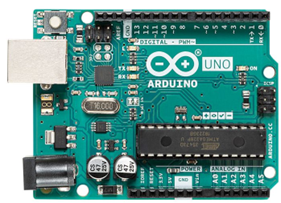
\includegraphics[width=7cm]{Digitalrechner_Arduino Uno.png}
    \end{center}
    \caption{Arduino}
\end{figure}

Auf dem Arduino ist ein Atmega328 Mikroprozessor verbaut, diese ist auf einer Platine beschaltet. Der Mikrocontroller kann direkt über eine serielle Schnittstelle geflasht werden. Es wird also kein externes Kompiliergerät benötigt. Mit der Arduino IDE lassen sich auf dem Arduino UNO rund 20 Pins programmieren. Bei einem Arduino UNO sind folgende Anschlüsse vorhanden: 

\begin{itemize}
    \item 13x digital Pins 
    \item 3x Timer 
    \item 6x PWM Pins 
    \item SDA und SCL Pins 
    \item 6x analog Pins 
    \item MISO MOSI Pins
\end{itemize}

Benutzt werden hierbei 5 der PWM-Pins, 4 der normalen Digital-Pins, die SDA- und SCL-Pins. Der USB-Anschluss wird lediglich zur Übertragung des Programms und zur Überwachung der korrekten Funktion während der Entwicklung benötigt.


\subsection{Steuerung}
Die Steuerung des Roboters erfolgt lediglich über die Motoren, welche mit unterschiedlichen PWM-Signalen neben vorwärtsn nach links und nach rechts gesteuert werden. 

\subsection{Regelung}
Die Regelung erfolgt über eine Kombination aus Kompass, den GPS-Koordinaten des Handys und den GPS-Koordinaten des GPS-Moduls, welches mit dem Arduino verbunden ist. Mittels der 2 Koordinatensets soll die Distanz zwischen den beiden Punkten errechnet werden, der Kompass gibt schliesslich die Richtung an, in welche es sich zu drehen gilt. Sobald die Distanz unter einen gewissen Schwellenwert fällt, wird die Position des Handy-GPS wieder überprüft und der Prozess beginnt von vorne.